% ============================================================================
% Generative AI -- Proof of Concept (PoC), Continuous Assessment-3
% Re-typeset from "CA 3_Generative_AI_Proof_of_Concept_Assessment_Template"
% (Template/ folder). Section order, numbering and headings follow the
% template exactly. Red "[TO BE FILLED: ...]" marks anything that is not
% available in the repository and must be supplied by the team.
% Build:  latexmk -pdf -interaction=nonstopmode main.tex   (uses biber)
% ============================================================================
\documentclass[11pt,letterpaper]{article}

\usepackage[T1]{fontenc}
\usepackage[utf8]{inputenc}
\usepackage{tgtermes}                 % Times-like serif, as in the template
\renewcommand{\ttdefault}{lmtt}
\usepackage[letterpaper,margin=1in]{geometry}
\usepackage{xcolor}
\usepackage{amssymb}
\usepackage{array}
\usepackage{tabularx}
\usepackage{booktabs}
\usepackage{graphicx}
\usepackage{caption}
\usepackage{float}
\usepackage{enumitem}
\usepackage{titlesec}
\usepackage{listings}
\usepackage{tikz}
\usetikzlibrary{arrows.meta,positioning,calc,fit,shapes.geometric}
\usepackage{microtype}
\usepackage[backend=biber,style=numeric,sorting=none,maxbibnames=10]{biblatex}
\addbibresource{references.bib}
\usepackage[hidelinks]{hyperref}
\usepackage{fancyhdr}
\usepackage{needspace}
\usepackage{longtable}

\setlength{\parindent}{0pt}
\setlength{\parskip}{5pt}
\setlength{\emergencystretch}{3em}
\renewcommand{\arraystretch}{1.25}
\pagestyle{fancy}\fancyhf{}\renewcommand{\headrulewidth}{0pt}
\cfoot{\small\thepage}

% Headings as in the template: bold "N. Title"; sub-headings "N.M Title".
\titleformat{\section}{\normalfont\bfseries\normalsize}{\thesection.}{0.4em}{}
\titleformat{\subsection}{\normalfont\bfseries\normalsize}{\thesubsection}{0.5em}{}
\titlespacing*{\section}{0pt}{14pt}{6pt}
\titlespacing*{\subsection}{0pt}{9pt}{4pt}

\captionsetup{font=small,labelfont=bf}

% Placeholder macro (visible, red).
\newcommand{\todo}[1]{\textcolor{red}{\textbf{[TO BE FILLED: #1]}}}
% Check boxes for the template's tick-lists.
\newcommand{\cbx}{$\square$}
\newcommand{\cbxx}{$\boxtimes$}

% Template tables use full borders and a bold header row.
\newcolumntype{L}[1]{>{\raggedright\arraybackslash}p{#1}}
\newcolumntype{Y}{>{\raggedright\arraybackslash}X}

% Listings
\lstdefinelanguage{TS}{
  keywords={const,let,return,if,else,function,export,type,interface,case,break,switch,try,catch,async,await,for,of,null,true,false},
  morecomment=[l]{//},morecomment=[s]{/*}{*/},morestring=[b]',morestring=[b]",
  sensitive=true}
\lstset{
  basicstyle=\ttfamily\scriptsize, keywordstyle=\bfseries\color{blue!60!black},
  commentstyle=\itshape\color{green!40!black}, stringstyle=\color{red!50!black},
  breaklines=true, breakatwhitespace=false, columns=fullflexible, keepspaces=true,
  frame=single, framerule=0.4pt, rulecolor=\color{black!40},
  numbers=left, numberstyle=\tiny\color{black!60}, numbersep=5pt,
  xleftmargin=14pt, framexleftmargin=14pt, aboveskip=6pt, belowskip=4pt,
  showstringspaces=false, tabsize=2, captionpos=b}

\begin{document}

% ------------------------------- Title block --------------------------------
\begin{center}
  {\bfseries\large GENERATIVE ARTIFICIAL INTELLIGENCE}\\[10pt]
  {\bfseries\large PROOF OF CONCEPT (PoC) --- CONTINUOUS ASSESSMENT-3}\\[8pt]
  {\small Semester VII --- Information Technology \,|\, Continuous Assessment \,|\, Maximum Marks: 10}
\end{center}

% ------------------------------ 1. Student Details --------------------------
\section{Student Details}
\begin{tabular}{|L{2.7in}|L{3.45in}|}
\hline
\textbf{Particular} & \textbf{Details}\\\hline
Student Name(s) & Chaitanya Kelkar; Jay Kerkar; Yash Kolekar\\\hline
Roll No(s) & 15; 16; 17 (respectively)\\\hline
Division & D20A\\\hline
Batch & A\\\hline
Faculty Name & Prof.\ Dipti Karani\\\hline
Date of Submission & 2 November 2026\\\hline
PoC Title & Crucible: An Agentic, Self-Healing Generative-AI Development Environment for Web3 dApps\\\hline
Selected Self-Learning Topic &
  \cbxx\ Prompt Engineering \quad \cbxx\ RAG Basics \quad
  \cbxx\ AI Hallucinations \& LLM Limitations \quad \cbxx\ Responsible AI \quad
  \cbxx\ Other: Agentic AI (tool-calling LLM agents over MCP)\\\hline
Individual / Group & Group (3 students)\\\hline
\end{tabular}

% ------------------------------ 2. Problem ----------------------------------
\section{Problem Identification}

\subsection{Problem Statement}
Building a decentralised application (dApp) today forces a developer to stitch together five disconnected tools: a code editor for Solidity and frontend code, a terminal running a local blockchain node, a browser to test the frontend, a wallet extension (with a manually configured RPC endpoint, imported keys and nonce resets), and a block explorer to debug failed transactions. These tools do not communicate with each other, and an ordinary AI coding assistant sees only text files: it has no awareness of chain state, wallet balances or deployment history, and it cannot observe a transaction revert, let alone repair it. Developers therefore spend more time wiring tools together than writing code, and Web3 development remains slow for experts and inaccessible to newcomers.\cite{crucible}

\subsection{Target Users}
Smart-contract and dApp developers, from beginners learning Solidity to experienced Web3 engineers who want faster build--test--debug cycles; hackathon and student teams prototyping on testnets.

\subsection{Why is this Problem Important?}
Smart-contract bugs are expensive and difficult to diagnose because contracts are immutable once deployed and failures surface as opaque transaction reverts. Shortening the loop \emph{write $\rightarrow$ compile $\rightarrow$ deploy $\rightarrow$ interact $\rightarrow$ debug} lowers the entry barrier to Web3, and an assistant that can observe execution results (instead of only emitting text) can catch and fix defects automatically before a developer wastes time on them. It also makes a concrete case study for tool-using generative-AI agents, where hallucinated output must be checked against ground truth produced by a compiler and an EVM.

% ------------------------------ 3. Solution ---------------------------------
\section{Proposed GenAI Solution}

\subsection{Proposed Solution}
\textbf{Crucible} is a browser-based agentic development environment: the user describes a dApp in natural language and a large language model (LLM) agent builds it step by step. The backend assembles a system prompt (role, tool documentation, workflows and a live index of workspace files) plus the chat history, and streams the request to an LLM through the Vercel AI SDK. The model acts only by calling tools exposed over the Model Context Protocol (MCP): writing files, compiling Solidity, starting a per-workspace Hardhat chain, deploying, calling contracts and recalling stored fixes. When a transaction reverts, a controller forces the model through a fixed seven-step repair sequence (snapshot, trace, recall, patch, compile, revert, redeploy) with at most three attempts. Every event is streamed to the browser so that all actions stay visible and overridable.

\medskip
\begin{tabular}{|L{2.1in}|L{4.05in}|}
\hline
\textbf{Item} & \textbf{Details}\\\hline
Primary GenAI Concept Used &
  Tool-using LLM agent \cite{yao2023react,schick2023toolformer} (function calling over MCP \cite{mcpspec}) steered by prompt engineering: a long role-and-workflow system prompt, plus per-step tool restriction (\texttt{activeTools} / forced \texttt{toolChoice}) that turns the model into a constrained self-repair state machine.\\\hline
Why was this concept selected? &
  Generating Solidity from text alone is unreliable. Grounding the LLM in real tool results (compiler errors, EVM traces, revert reasons) lets the system detect hallucinated or buggy code automatically and correct it, instead of trusting the first answer. MCP gives a uniform, schema-validated way to expose chain, compiler, wallet and memory services to the model.\\\hline
Expected Input / Output &
  \textbf{Input:} a natural-language request (e.g.\ ``Build me a token vault with deposit, withdraw and a 24-hour withdrawal cooldown'') together with the current workspace files and chat history. \textbf{Output:} Solidity and frontend source files written to the workspace, compiled artifacts, deployed contract addresses, a live dApp preview, and a streamed trace of every tool call, revert and patch.\\\hline
\end{tabular}

\medskip
\textbf{Syllabus mapping.} The PoC covers: Module 1 (NLP applications, transformer/GPT overview, pre-trained models used through prompting rather than fine-tuning, GPT-based dialogue system); Module 2 (text/code generation, transfer learning, privacy and security); Module 5 (prompt engineering, RAG-style retrieval of past fixes from memory, hallucinations and LLM limitations, conversational AI); Module 6 (developer-tooling case study, zero/few-shot use, agentic AI trends, Responsible AI). Modules 3 (autoencoders, VAEs) and 4 (GANs) are not covered.

% ------------------------------ 4. Architecture -----------------------------
\section{System Architecture / Workflow}

Figure~\ref{fig:arch} follows the suggested flow of the template (User/Input $\rightarrow$ Preprocessing $\rightarrow$ GenAI Model $\rightarrow$ Processing $\rightarrow$ Output $\rightarrow$ Evaluation). Steps are numbered in execution order.

\begin{figure}[H]
\centering
\resizebox{\textwidth}{!}{%
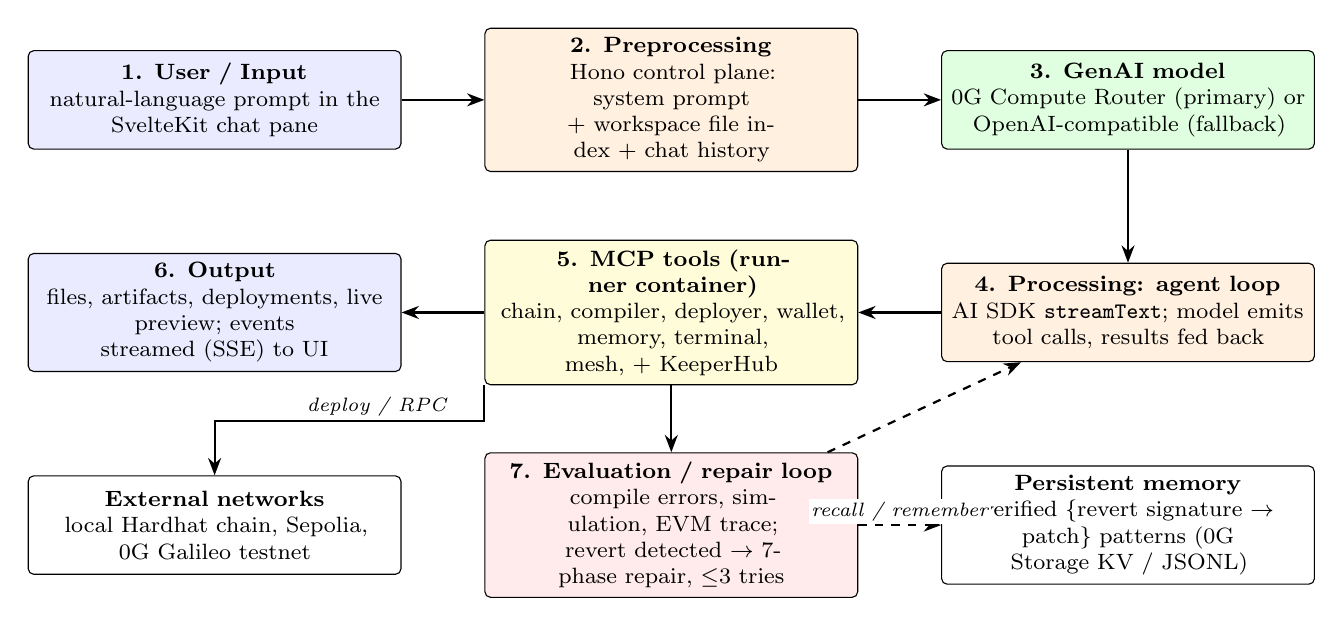
\begin{tikzpicture}[
  font=\footnotesize,
  box/.style={draw, rounded corners=2pt, align=center, minimum height=1.25cm, text width=4.5cm, fill=#1},
  box/.default=white,
  arr/.style={-{Stealth[length=2.2mm]}, thick},
  darr/.style={-{Stealth[length=2.2mm]}, thick, dashed},
  lab/.style={font=\scriptsize\itshape, fill=white, inner sep=1pt}]
% Row 1 (left to right)
\node[box=blue!8]   (A) at (0,0)    {\textbf{1. User / Input}\\ natural-language prompt in the\\ SvelteKit chat pane};
\node[box=orange!12](B) at (5.8,0)  {\textbf{2. Preprocessing}\\ Hono control plane: system prompt\\ + workspace file index + chat history};
\node[box=green!12] (C) at (11.6,0) {\textbf{3. GenAI model}\\ 0G Compute Router (primary) or\\ OpenAI-compatible (fallback)};
% Row 2 (right to left)
\node[box=orange!12](D) at (11.6,-2.7) {\textbf{4. Processing: agent loop}\\ AI SDK \texttt{streamText}; model emits\\ tool calls, results fed back};
\node[box=yellow!15](E) at (5.8,-2.7)  {\textbf{5. MCP tools (runner container)}\\ chain, compiler, deployer, wallet,\\ memory, terminal, mesh, + KeeperHub};
\node[box=blue!8]   (F) at (0,-2.7)    {\textbf{6. Output}\\ files, artifacts, deployments, live\\ preview; events streamed (SSE) to UI};
% Row 3
\node[box=red!8]    (G) at (5.8,-5.4)  {\textbf{7. Evaluation / repair loop}\\ compile errors, simulation, EVM trace;\\ revert detected $\rightarrow$ 7-phase repair, $\le$3 tries};
\node[box=white]    (H) at (0,-5.4)    {\textbf{External networks}\\ local Hardhat chain, Sepolia,\\ 0G Galileo testnet};
\node[box=white]    (I) at (11.6,-5.4) {\textbf{Persistent memory}\\ verified \{revert signature $\rightarrow$\\ patch\} patterns (0G Storage KV / JSONL)};
\draw[arr] (A)--(B); \draw[arr] (B)--(C); \draw[arr] (C)--(D);
\draw[arr] (D)--(E); \draw[arr] (E)--(F);
\draw[arr] (E)--(G); \draw[darr] (G)--(D);
\draw[arr] (E.south west)--++(0,-0.45)-|(H.north) node[lab,pos=0.2,above]{deploy / RPC};
\draw[darr] (G)--(I) node[lab,midway,above]{recall / remember};
\end{tikzpicture}}
\caption{System architecture and workflow of the Crucible PoC. Solid arrows show the main request flow; dashed arrows show the repair feedback and memory lookups.}
\label{fig:arch}
\end{figure}

Figure~\ref{fig:repair} details the signature mechanism of the PoC. A revert returned by \texttt{deploy\_local}, \texttt{call\_contract} or \texttt{send\_tx\_local} starts a controller that, at every model step, exposes \emph{only one} tool and forces the model to call it, so the model cannot skip or reorder the repair phases. A successful verification emits \texttt{patch\_verified} and allows one constrained ``resume'' step so the original task continues; a fourth failed attempt emits \texttt{repair\_failed} and ends the turn.

\begin{figure}[H]
\centering
\resizebox{\textwidth}{!}{%
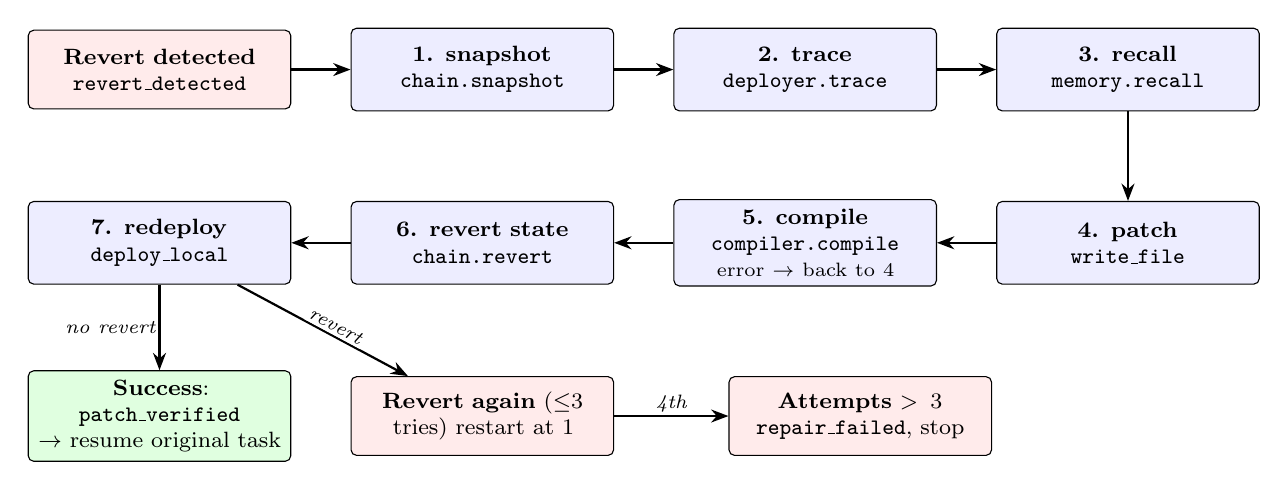
\begin{tikzpicture}[
  font=\footnotesize,
  ph/.style={draw, rounded corners=2pt, align=center, minimum height=1.05cm, text width=3.1cm, fill=blue!7},
  ev/.style={draw, rounded corners=2pt, align=center, minimum height=1.0cm, text width=3.1cm, fill=red!8},
  ok/.style={draw, rounded corners=2pt, align=center, minimum height=1.0cm, text width=3.1cm, fill=green!12},
  arr/.style={-{Stealth[length=2.2mm]}, thick},
  lab/.style={font=\scriptsize\itshape, fill=white, inner sep=1pt}]
\node[ev] (R) at (0,0)    {\textbf{Revert detected}\\ \texttt{revert\_detected}};
\node[ph] (P1) at (4.1,0) {\textbf{1. snapshot}\\ \texttt{chain.snapshot}};
\node[ph] (P2) at (8.2,0) {\textbf{2. trace}\\ \texttt{deployer.trace}};
\node[ph] (P3) at (12.3,0){\textbf{3. recall}\\ \texttt{memory.recall}};
\node[ph] (P4) at (12.3,-2.2){\textbf{4. patch}\\ \texttt{write\_file}};
\node[ph] (P5) at (8.2,-2.2) {\textbf{5. compile}\ \texttt{compiler.compile}\ {\scriptsize error $\rightarrow$ back to 4}};
\node[ph] (P6) at (4.1,-2.2) {\textbf{6. revert state}\\ \texttt{chain.revert}};
\node[ph] (P7) at (0,-2.2)   {\textbf{7. redeploy}\\ \texttt{deploy\_local}};
\node[ok] (OK) at (0,-4.4)   {\textbf{Success}: \texttt{patch\_verified}\\ $\rightarrow$ resume original task};
\node[ev] (FL) at (4.1,-4.4) {\textbf{Revert again}\ ($\le$3 tries) restart at 1};
\node[ev] (RF) at (8.9,-4.4) {\textbf{Attempts $>3$}\\ \texttt{repair\_failed}, stop};
\draw[arr] (R)--(P1); \draw[arr] (P1)--(P2); \draw[arr] (P2)--(P3);
\draw[arr] (P3)--(P4); \draw[arr] (P4)--(P5); \draw[arr] (P5)--(P6); \draw[arr] (P6)--(P7);
\draw[arr] (P7)--(OK) node[lab,midway,left]{no revert};
\draw[arr] (P7)--(FL) node[lab,pos=0.55,above,sloped]{revert};
\draw[arr] (FL)--(RF) node[lab,midway,above]{4th};


\end{tikzpicture}}
\caption{Forced seven-phase self-healing repair loop implemented in \texttt{packages/agent/src/loop.ts}.}
\label{fig:repair}
\end{figure}

% ------------------------------ 5. Tools ------------------------------------
\Needspace{14\baselineskip}
\section{Tools, Technologies and Model}
Versions are the semantic-version ranges declared in the repository's \texttt{package.json} files.

\medskip
\begin{tabular}{|L{1.9in}|L{4.25in}|}
\hline
\textbf{Component} & \textbf{Technology Used}\\\hline
Programming Language & TypeScript (\texttt{typescript} \texttt{\^{}}5.7.3) executed directly by Bun 1.3.6; Solidity 0.8.x \cite{solidity} for the generated contracts; JavaScript/Svelte for the generated frontend\\\hline
GenAI Model & Transformer-based \cite{vaswani2017attention} chat-completion LLM selected at run time through environment variables: primary model from the 0G Compute Router (\texttt{OG\_MODEL}; the project documentation cites \texttt{qwen3.6-plus} and \texttt{GLM-5-FP8} as examples), or any model on an OpenAI-compatible endpoint (\texttt{OPENAI\_MODEL}) as a degraded-mode fallback. No model is trained or fine-tuned in this project.\\\hline
Framework / Library & Vercel AI SDK \cite{aisdk} (\texttt{ai} \texttt{\^{}}6.0.168, \texttt{@ai-sdk/openai} \texttt{\^{}}3, \texttt{@ai-sdk/mcp} \texttt{\^{}}1.0.36); MCP server SDK (\texttt{@modelcontextprotocol/server} 2.0.0-alpha.2); Hono \texttt{\^{}}4.12; Zod \texttt{\^{}}4; viem \texttt{\^{}}2.48; Hardhat \cite{hardhat} \texttt{\^{}}3; Prisma \texttt{\^{}}7.8; better-auth \texttt{\^{}}1.6 (Sign-In with Ethereum); dockerode; Turborepo \texttt{\^{}}2.5\\\hline
Dataset / Documents & No training dataset. Inputs at run time are the user's prompts, the workspace files, and the persisted chat history. A store of verified ``revert signature $\rightarrow$ patch'' patterns acts as the agent's memory (0G Storage KV when configured, otherwise a local JSONL file); \texttt{scripts/seed-memories.sh} seeds demo patterns.\\\hline
API / Platform & 0G Compute Router \cite{ogrouter} (OpenAI-compatible REST); KeeperHub hosted MCP (post-deploy automation); Docker (one runner container per workspace); PostgreSQL; local Hardhat chain, Sepolia and 0G Galileo testnets\\\hline
User Interface & SvelteKit \texttt{\^{}}2.57 / Svelte \texttt{\^{}}5.55 web app with Tailwind CSS \texttt{\^{}}4.2, chat rail, CodeMirror 6 editor, live preview iframe, transaction inspector and an xterm.js \texttt{\^{}}6 terminal\\\hline
Other Tools & Bun test runner, ESLint, Prettier, GitHub Actions CI, Vite \texttt{\^{}}8 (per-workspace preview server), Portless local URLs\\\hline
\end{tabular}

% ------------------------------ 6. Implementation ---------------------------
\section{Implementation}

\subsection{Implementation Steps}
\begin{enumerate}[leftmargin=1.6em,itemsep=3pt]
  \item \textbf{Workspace provisioning.} The backend (\texttt{packages/backend}, Hono + Prisma) creates a real directory \texttt{contracts/}, \texttt{frontend/}, \texttt{.crucible/} per workspace, starts one Docker runner container hosting the MCP servers, and a Vite preview server. Access is gated by Sign-In with Ethereum sessions \cite{eip4361}.
  \item \textbf{Prompt assembly.} On \texttt{POST /api/prompt}, \texttt{buildSystemPrompt()} creates the system prompt (role, tool catalogue, local/0G/Sepolia/KeeperHub workflows, repair rules, mesh rules) and appends an index of current workspace files with SHA-256 prefixes; the persisted chat history is replayed as prior messages.
  \item \textbf{Streaming inference with tool calling.} \texttt{runAgentTurn()} opens an MCP client per runner service and calls \texttt{streamText} (up to 40 steps) against the selected provider. A fetch wrapper normalises provider quirks (empty tool-call types, \texttt{reasoning\_content}) and classifies 0G Router failures (rate limit, exhausted balance, outage) so the UI can show an honest fallback state.
  \item \textbf{Tool execution.} The model writes Solidity/frontend files, compiles (\texttt{compiler.compile}), deploys (\texttt{deploy\_local},\texttt{deploy\_sepolia}, \texttt{deploy\_og\_chain}), interacts (\texttt{wallet.call\_contract}) and advances chain time (\texttt{chain.mine}); every tool call and result is emitted as a typed event over SSE.
  \item \textbf{Self-healing and memory.} Reverts are detected by parsing tool results; \texttt{prepareStep} then restricts the model to the single tool of the current repair phase, a verified patch is stored through \texttt{memory.remember}, and one resume step returns control to the original task. A cleanup \texttt{finally} block reverts the chain snapshot if a turn is cancelled mid-repair.
\end{enumerate}

\subsection{Important Code / Algorithm}
Listing~\ref{lst:phase} shows how the repair state machine constrains the model (abridged from \texttt{packages/agent/\allowbreak src/loop.ts}; type casts and comments omitted). Listing~\ref{lst:detect} shows how a revert is distinguished from an infrastructure error, and Algorithm~\ref{alg:repair} gives the controller in pseudocode.

\begin{lstlisting}[language=TS,caption={Per-phase tool restriction and forced tool choice (abridged).},label={lst:phase}]
const REPAIR_PHASE_TOOLS = {
  snapshot: { activeTools: ['snapshot'],     toolName: 'snapshot' },
  trace:    { activeTools: ['trace'],        toolName: 'trace' },
  recall:   { activeTools: ['recall'],       toolName: 'recall' },
  patch:    { activeTools: ['write_file'],   toolName: 'write_file' },
  compile:  { activeTools: ['compile'],      toolName: 'compile' },
  revert:   { activeTools: ['revert'],       toolName: 'revert' },
  deploy:   { activeTools: ['deploy_local'], toolName: 'deploy_local' },
};
...
streamText({
  model: openai.chat(config.model),
  system: buildSystemPrompt(files),
  stopWhen: [stepCountIs(40), () => repairFailed],
  prepareStep: ({ experimental_context }) => {
    ...
    const phaseConfig = REPAIR_PHASE_TOOLS[repairCtx.phase];
    return {
      activeTools: phaseConfig.activeTools,
      toolChoice: { type: 'tool', toolName: phaseConfig.toolName },
      experimental_context: repairCtx,
    };
  },
  ...
});
\end{lstlisting}

\begin{lstlisting}[language=TS,caption={Revert detection: only genuine EVM reverts start the repair loop (abridged).},label={lst:detect}]
export function extractDeployRevert(toolName: string, toolResult: unknown) {
  if (toolName !== 'deploy_local') return { reverted: false };
  const raw = toolResult as { isError?: boolean;
    content?: Array<{ type: string; text?: string }> };
  if (!raw.isError) return { reverted: false };
  const message = raw.content?.filter((c) => c.type === 'text')
    .map((c) => c.text ?? '').join('\n') ?? '';
  // Infrastructure errors ("node not running", "not found in artifact
  // store") must not trigger the repair loop.
  if (!/revert/i.test(message)) return { reverted: false };
  const txHash = /0x[0-9a-f]{64}/i.exec(message)?.[0] ?? '0x' + '0'.repeat(64);
  const reason = /reverted with reason:\s*"([^"]+)"/i.exec(message)?.[1];
  return { reverted: true, txHash, revertSignature: reason ?? message.slice(0, 200) };
}
\end{lstlisting}

\begin{figure}[H]
\centering
\begin{minipage}{0.93\textwidth}
\begin{lstlisting}[basicstyle=\ttfamily\scriptsize,numbers=none,xleftmargin=0pt,framexleftmargin=4pt,caption={Repair-loop controller (pseudocode of \texttt{runAgentTurn}).},label={alg:repair}]
on tool result r of deploy_local / call_contract / send_tx_local:
    if r is a genuine EVM revert:
        if no repair active:  start repair (attempts = 1); emit revert_detected
        else:                 attempts += 1
        if attempts > 3:      emit repair_failed; stop turn
        else:                 phase = snapshot
for each model step while phase != idle:
    restrict tools to TOOL[phase] and force the call
    snapshot -> trace -> recall -> patch(write_file) -> compile
        (compile error -> phase = patch) -> chain.revert -> redeploy
    on redeploy success: emit patch_verified; phase = resume (one step)
    on redeploy revert:  attempts += 1 (see above)
\end{lstlisting}
\end{minipage}
\end{figure}

% ------------------------------ 7. Demonstration ----------------------------
\section{Working Demonstration}

\begin{figure}[H]
\centering
\begin{minipage}[t]{0.485\textwidth}
\vspace{0pt}\centering
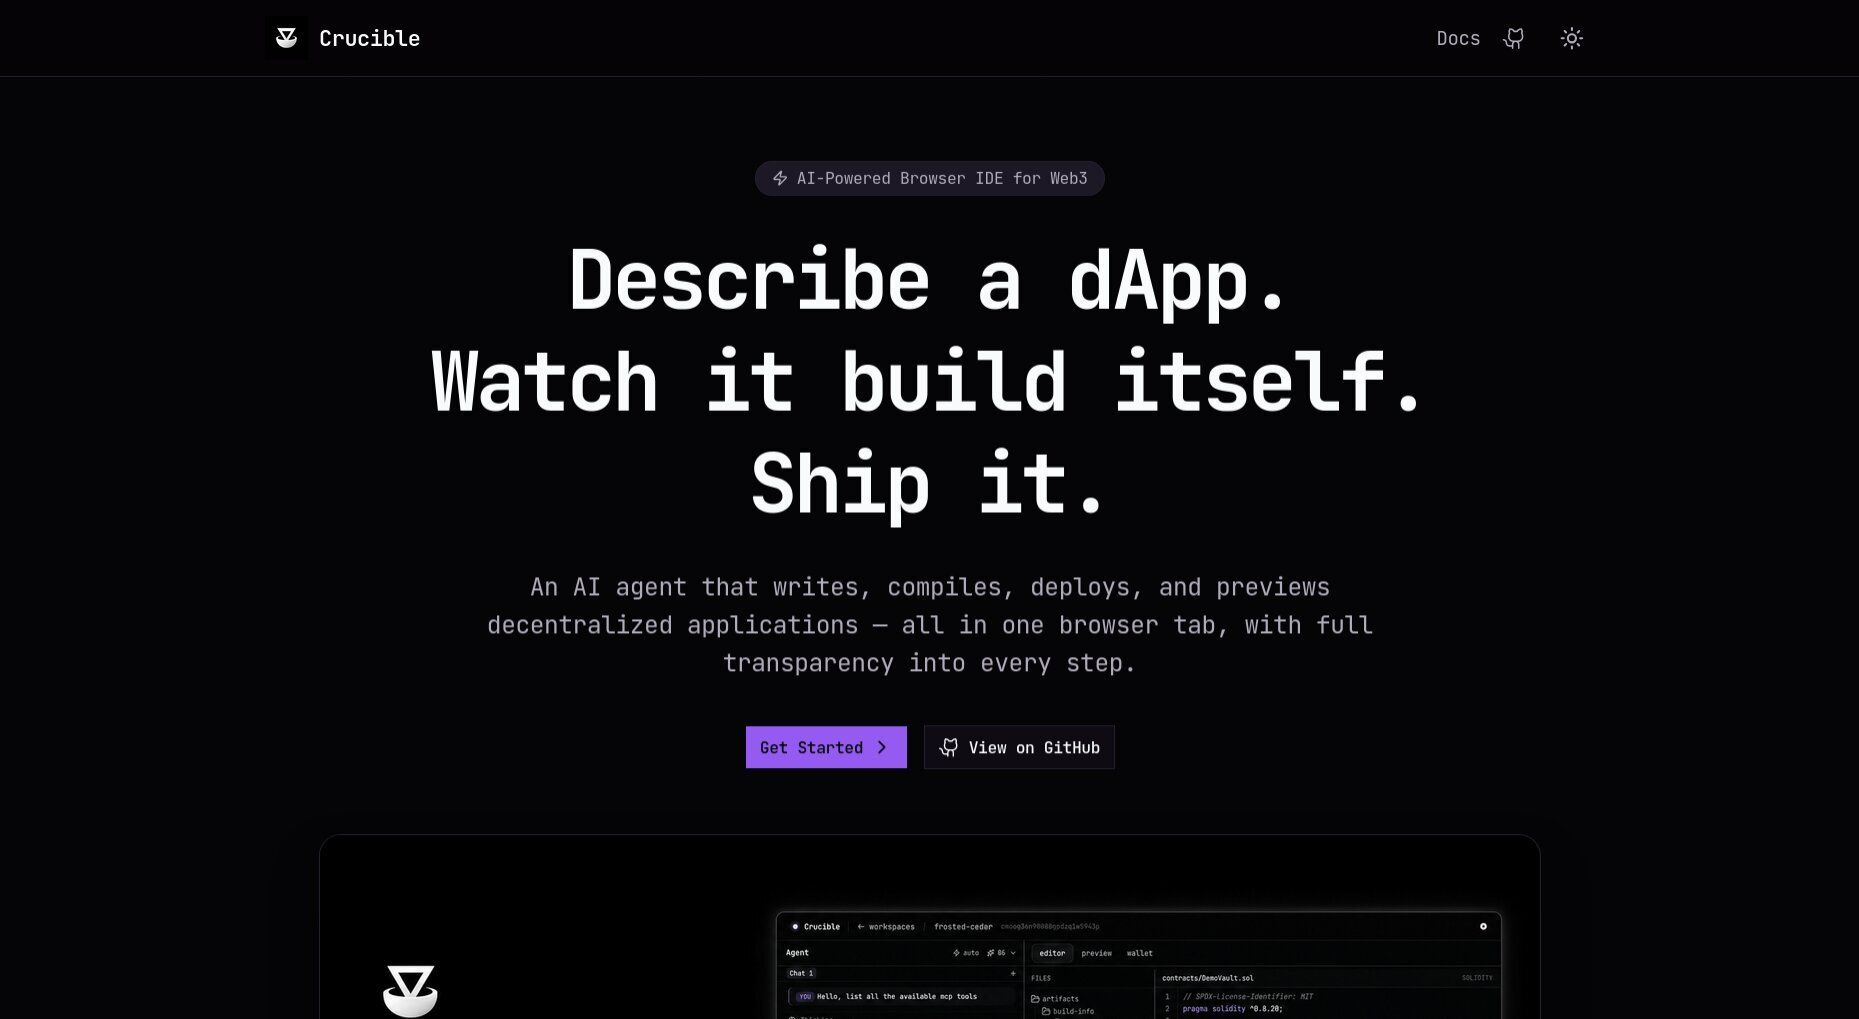
\includegraphics[width=\linewidth]{figures/site_1.jpeg}
\captionof{figure}{Crucible landing page.}
\end{minipage}\hfill
\begin{minipage}[t]{0.485\textwidth}
\vspace{0pt}\centering
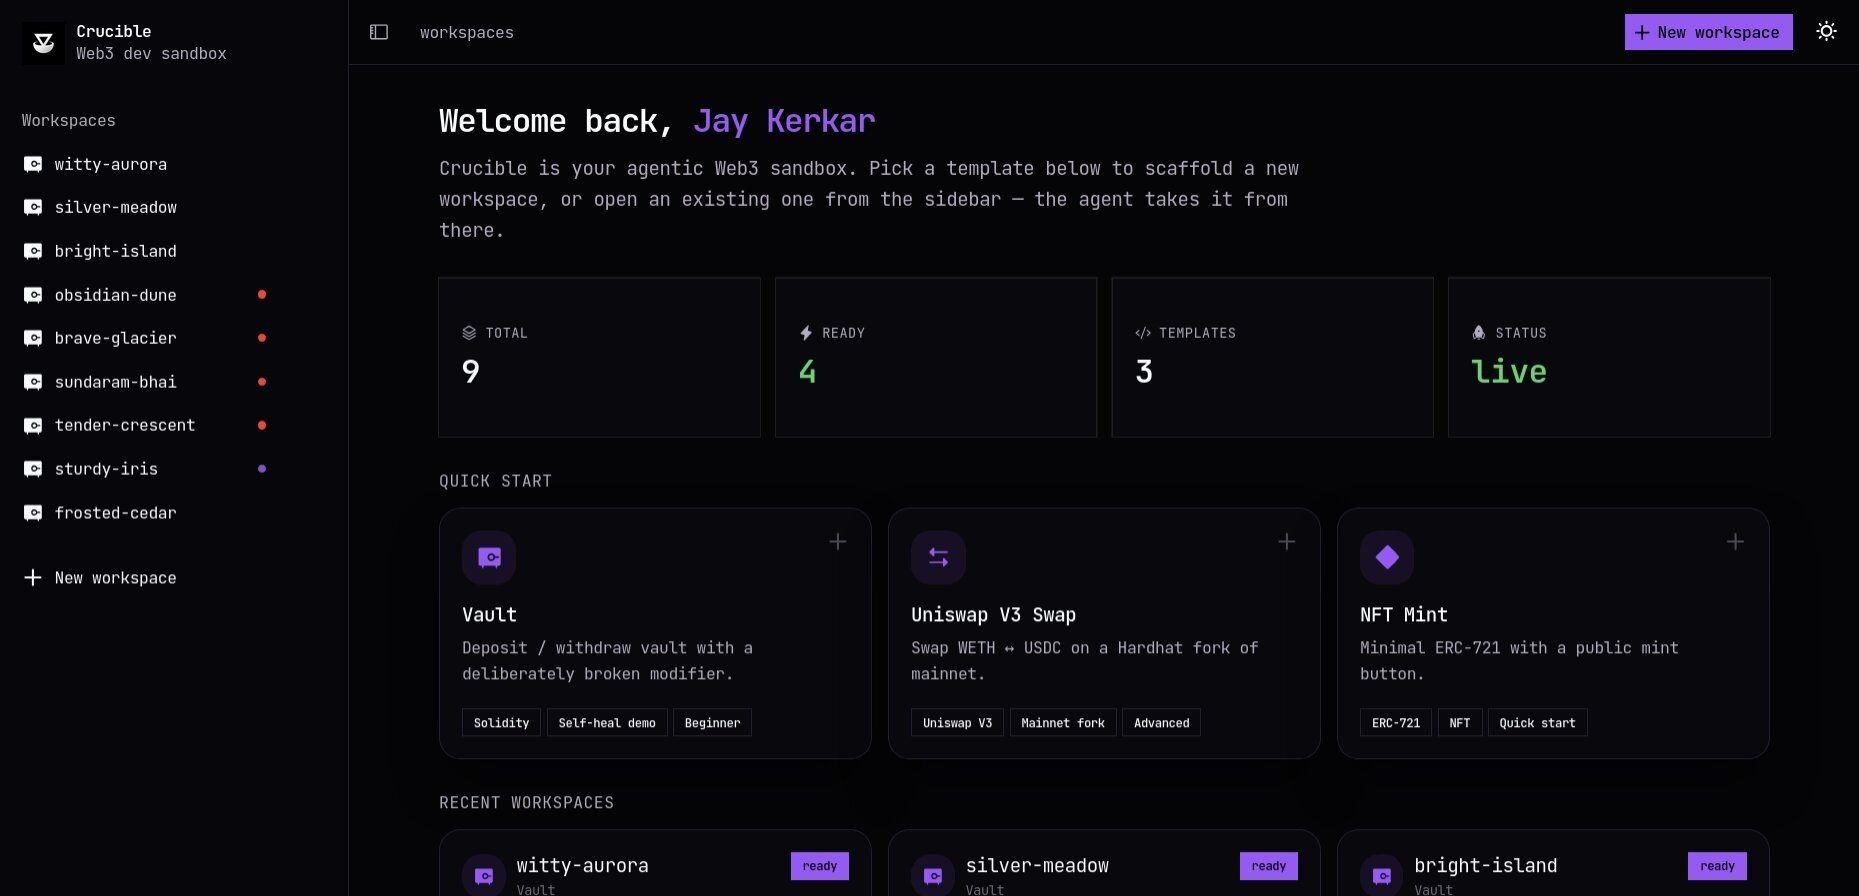
\includegraphics[width=\linewidth]{figures/site_2.jpeg}
\captionof{figure}{Workspace dashboard with the three starter templates.}
\end{minipage}
\end{figure}

\begin{figure}[H]
\centering
\begin{minipage}[t]{0.485\textwidth}
\vspace{0pt}\centering
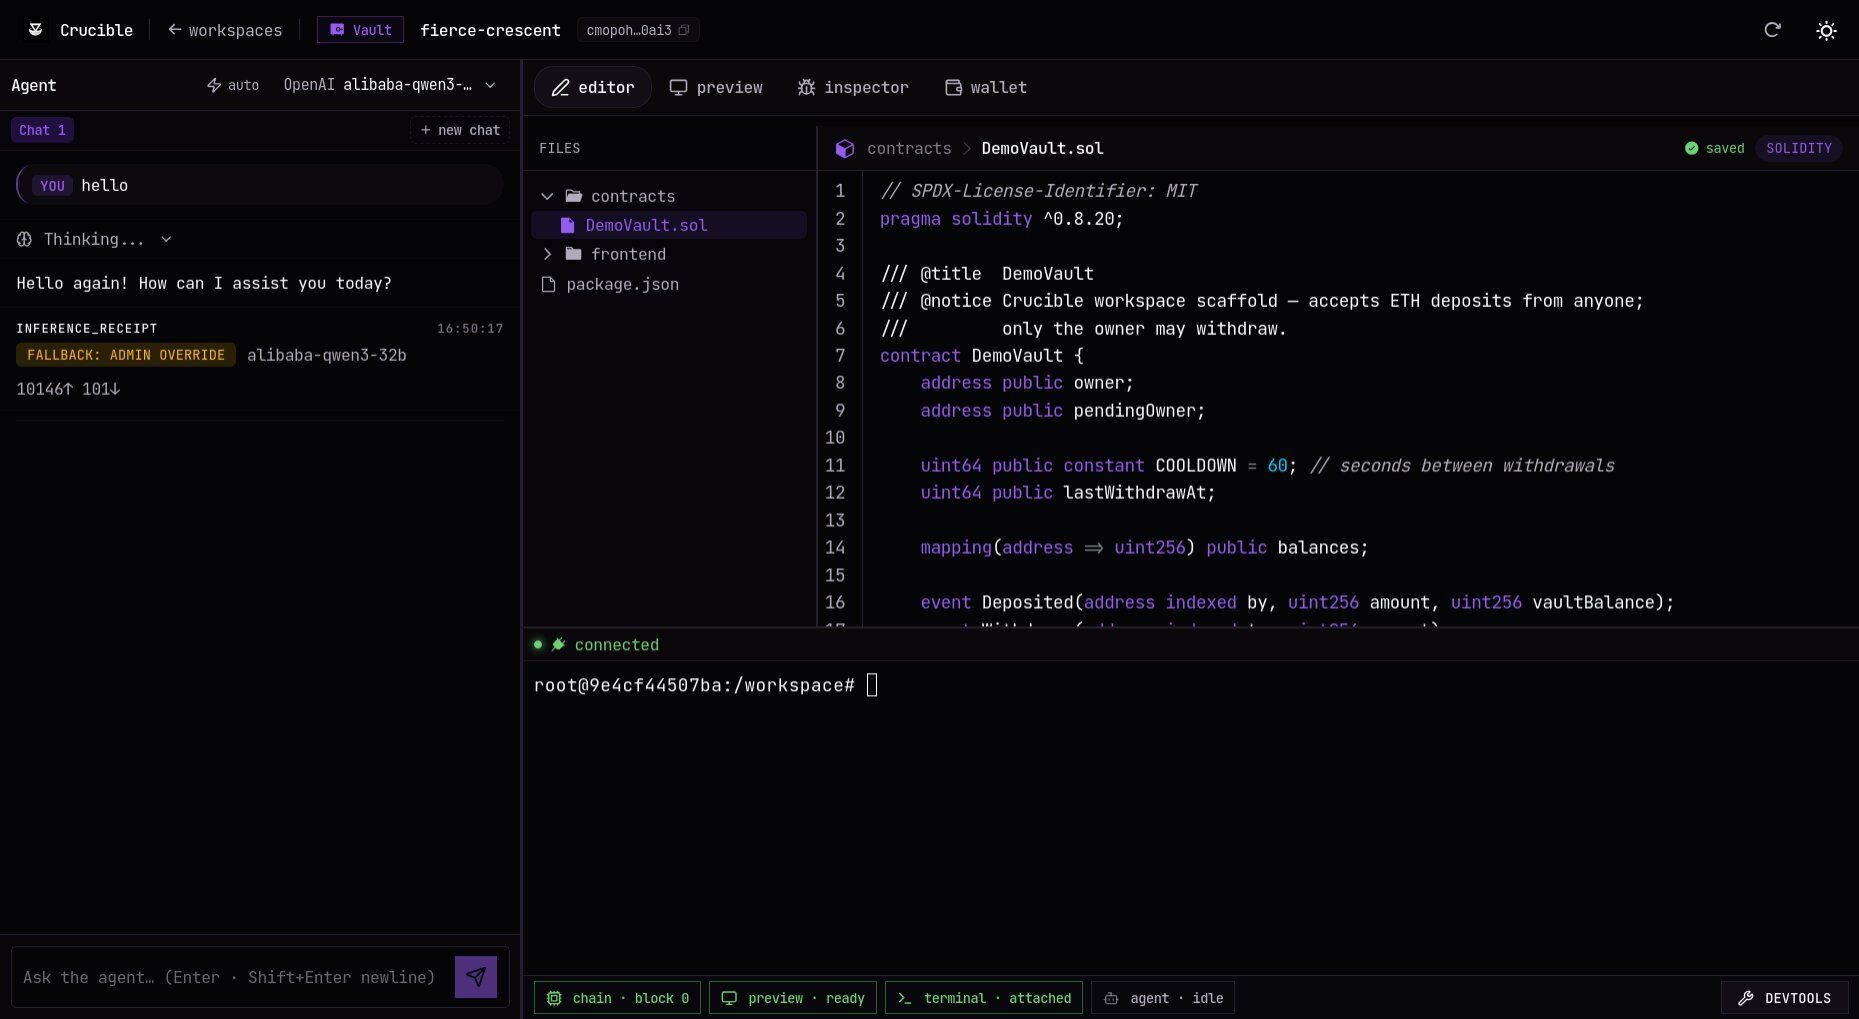
\includegraphics[width=\linewidth]{figures/site_4.jpeg}
\captionof{figure}{\textbf{Screenshot 1 --- Input.} Agent workspace: prompt in the chat rail, generated \texttt{DemoVault.sol} in the editor, workspace terminal.}
\end{minipage}\hfill
\begin{minipage}[t]{0.485\textwidth}
\vspace{0pt}\centering
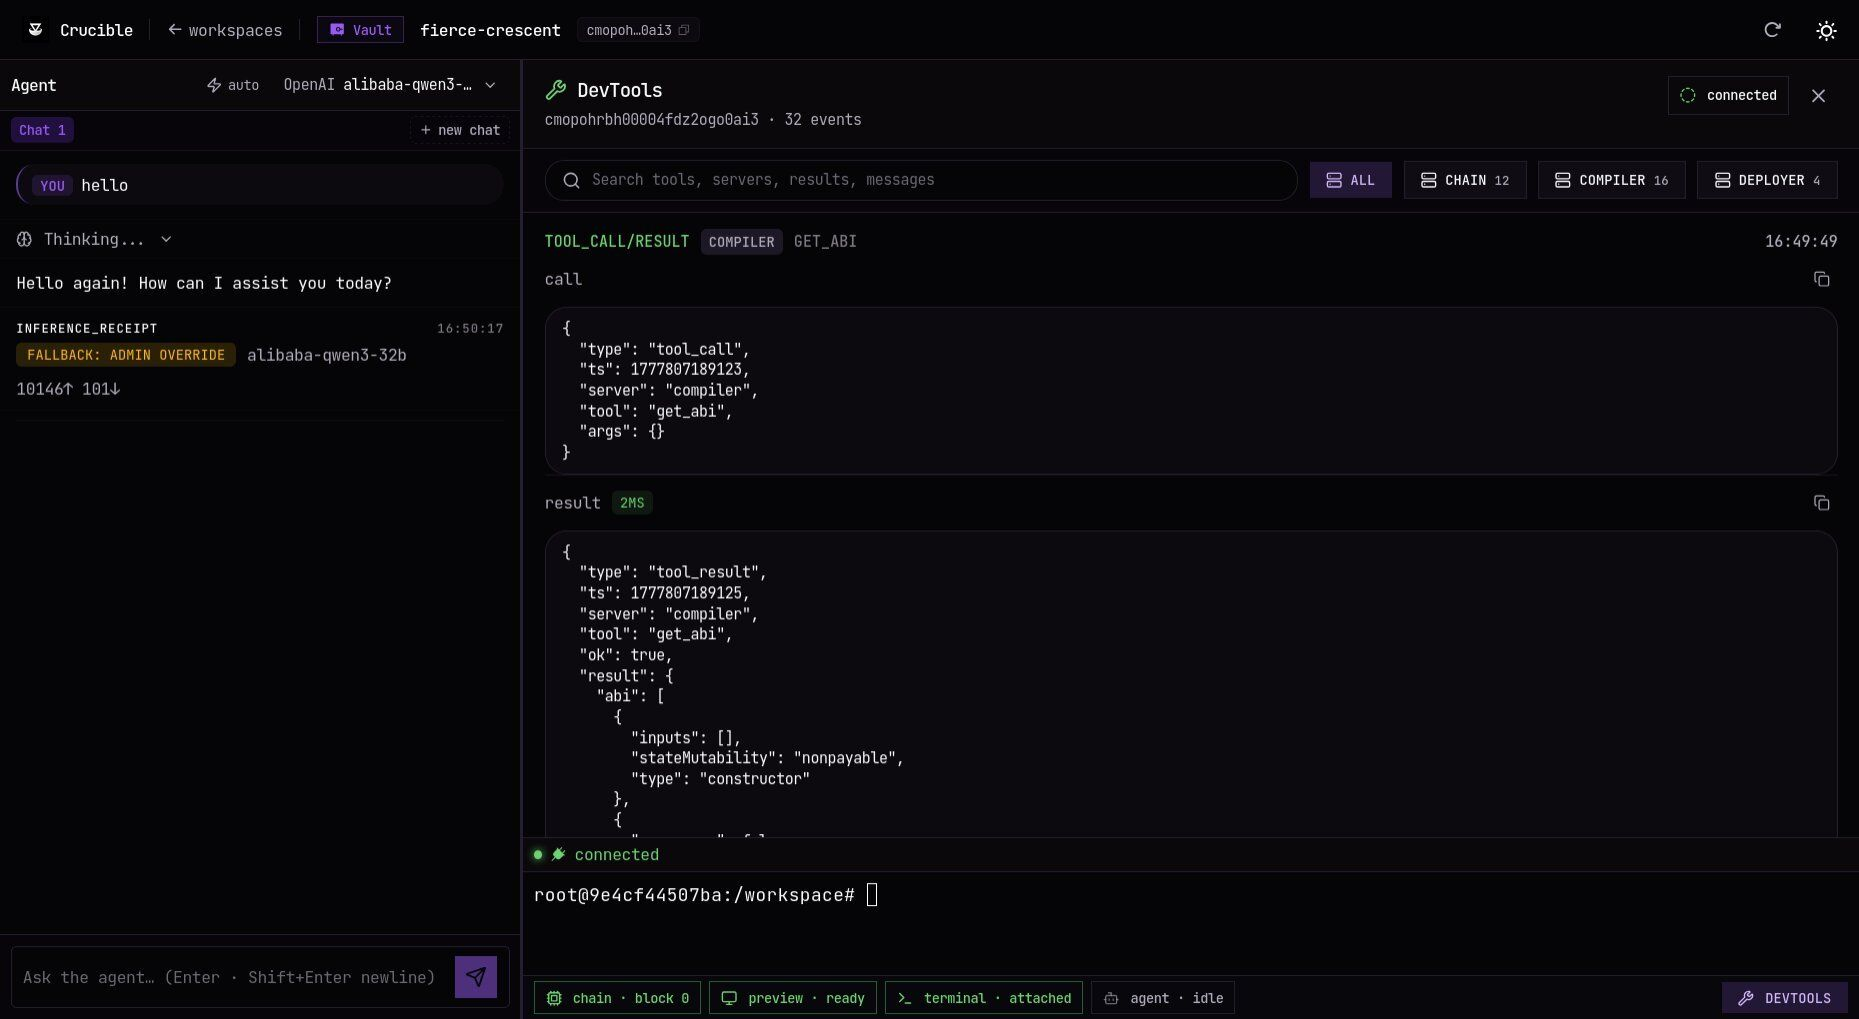
\includegraphics[width=\linewidth]{figures/site_6.jpeg}
\captionof{figure}{\textbf{Screenshot 2 --- Processing / Model.} DevTools inspector: \texttt{tool\_call}/\texttt{tool\_result} pair and inference receipt.}
\end{minipage}
\end{figure}

\begin{figure}[H]
\centering
\begin{minipage}[t]{0.485\textwidth}
\vspace{0pt}\centering
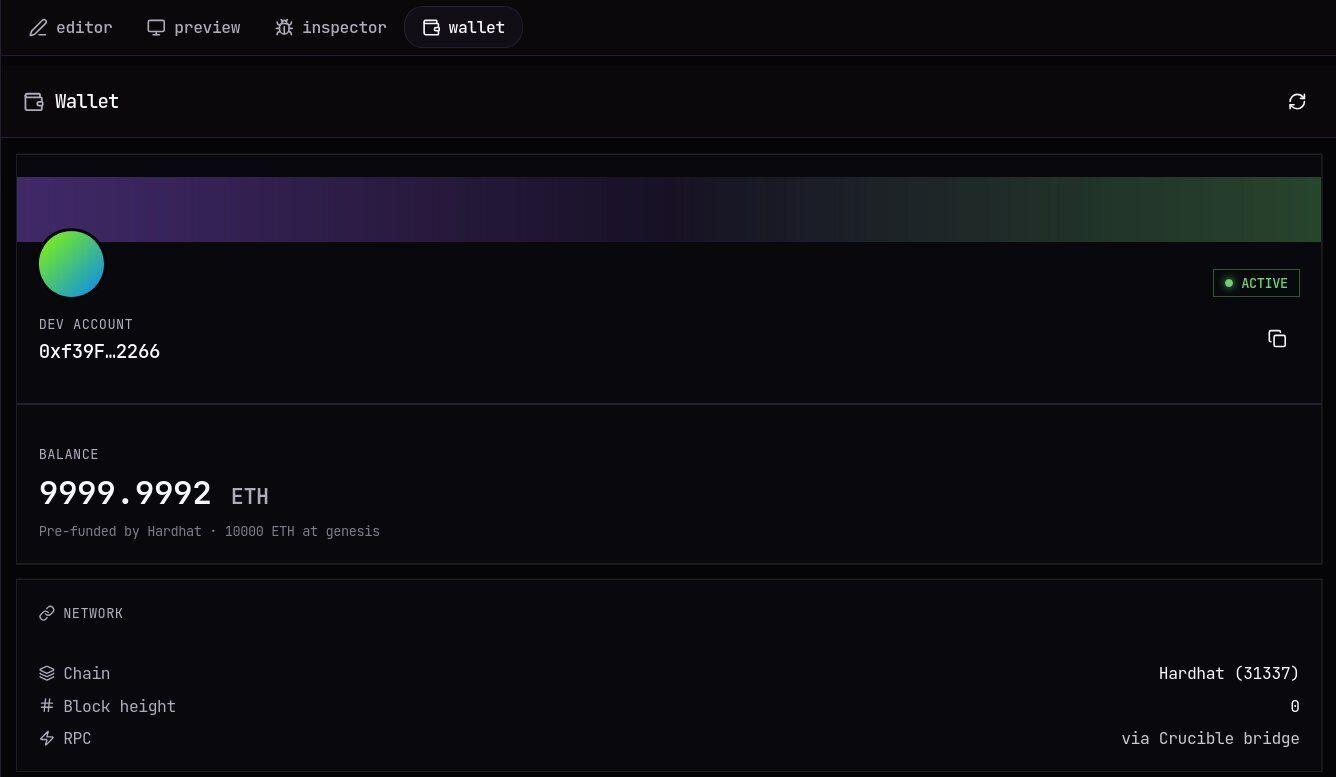
\includegraphics[width=\linewidth]{figures/site_5.jpeg}
\captionof{figure}{\textbf{Screenshot 3 --- Output.} Embedded dev wallet on the workspace's local Hardhat chain.}
\end{minipage}\hfill
\begin{minipage}[t]{0.485\textwidth}
\vspace{0pt}\centering
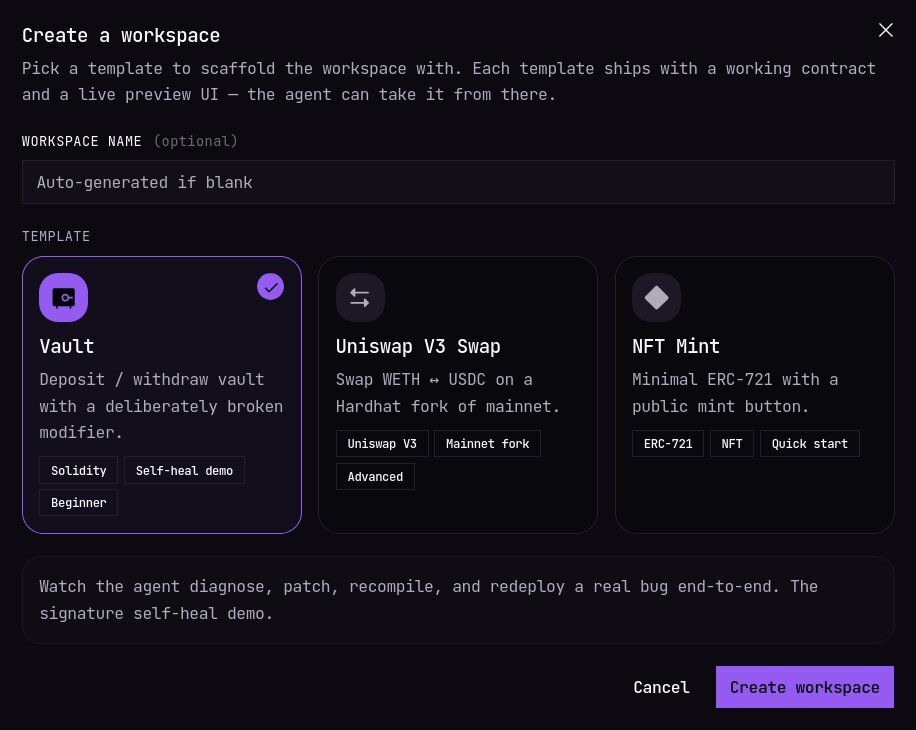
\includegraphics[width=\linewidth]{figures/site_3.jpeg}
\captionof{figure}{Create-workspace dialog with the Vault self-heal template.}
\end{minipage}
\end{figure}

\textbf{How to run the PoC} (from the repository's \texttt{README.md} and \texttt{packages/backend/.env.example}):
\begin{enumerate}[leftmargin=1.6em,itemsep=1pt,topsep=2pt]
  \item Clone the repository and copy the backend environment template to \texttt{.env}.
  \item Set the inference credentials: \texttt{OG\_API\_KEY} and \texttt{OG\_MODEL} (0G Compute Router), or \texttt{OPENAI\_BASE\_URL}, \texttt{OPENAI\_API\_KEY} and \texttt{OPENAI\_MODEL} (fallback); also set \texttt{DATABASE\_URL} and \texttt{BETTER\_AUTH\_SECRET}.
  \item Build the runtime image: \texttt{bun run -{}-cwd packages/backend runtime:build}.
  \item Run \texttt{bun install}, then \texttt{bun run dev}, and open the app in the browser.
\end{enumerate}

\textbf{Demo / GitHub / Google Colab / Drive / Video Link:}\\ Source repository: \url{https://github.com/WhyAsh5114/Crucible}\\ Demo video (YouTube): \url{https://www.youtube.com/watch?v=XDz7qSXFfp8}

% ------------------------------ 8. Results ----------------------------------
\section{Results and Evaluation}

\subsection{Test Cases}
The repository's automated unit tests for the agent package (\texttt{packages/agent/test}) were run with \texttt{bun test}. Five representative cases are listed; the whole run reported 40 passed, 0 failed (69 assertions, 3 test files). See Section~8.3 for how the run was performed.

\medskip
\small
\begin{tabular}{|c|L{1.5in}|L{1.5in}|L{1.2in}|c|}
\hline
\textbf{Test Case} & \textbf{Input} & \textbf{Expected Output} & \textbf{Actual Output} & \textbf{Result}\\\hline
1 & \texttt{extractDeployRevert} on a \texttt{deploy\_local} error ``Transaction reverted: 0xaaa\ldots\ reverted with reason: "Ownable: caller is not the owner"'' & \texttt{reverted: true}, tx hash extracted, signature = \texttt{Ownable: caller is not the owner} & Matched expected & Pass\\\hline
2 & \texttt{extractDeployRevert} on error text ``node not running'' (infrastructure error) & \texttt{reverted: false} (repair loop must not start) & Matched expected & Pass\\\hline
3 & \texttt{extractSnapshotId} on tool text \texttt{\{"snapshotId":\allowbreak"snap\_42"\}} & \texttt{"snap\_42"} & Matched expected & Pass\\\hline
4 & \texttt{extractSendTxRevert} on a \texttt{send\_tx\_local} result with \texttt{status: "reverted"} & \texttt{reverted: true}, signature contains ``transaction reverted'' & Matched expected & Pass\\\hline
5 & \texttt{classifyRouterError} with HTTP 429, 402 and 500 from the 0G Router & \texttt{rate\_limited}, \texttt{balance\_exhausted}, \texttt{provider\_unavailable} & Matched expected & Pass\\\hline
\end{tabular}
\normalsize

\subsection{Evaluation Criteria}
\cbxx\ Accuracy (rule-based revert detection and error classification) \quad
\cbxx\ Response Time (tool-pipeline latency, Table~\ref{tab:bench}) \quad
\cbxx\ Other: functional correctness of the repair-loop logic (automated unit tests).

\subsection{Results and Observations}
The 40 unit tests of the agent package pass. They cover revert detection (including the rule that infrastructure errors never trigger a repair), snapshot and deployment metadata extraction, 0G Router error classification and trace filtering, and the content of the generated system prompt. The run was performed on 2 November 2026 using Bun 1.4.2 on a scratch copy of \texttt{packages/agent} and \texttt{packages/types} with dependencies resolved afresh, because \texttt{bun install -{}-frozen-lockfile} on the repository itself reported that \texttt{bun.lock} was out of date. The backend, frontend and other MCP packages also contain tests, but they were not run for this report (the backend tests need a PostgreSQL instance).

The tests exercise the helper functions only: the repository itself notes that integration tests of the full revert-triggers-loop and three-failure-cap behaviour require mocking \texttt{streamText} and are out of scope of the current tests. The repository contains no systematic end-to-end benchmark of the generative component (e.g.\ fraction of prompts producing a compiling, deployable contract, repair success rate or hallucination rate), so none is claimed here.

\textbf{Observations from the running instance} (values read from the screenshots in Section~7): the workspace dashboard lists 9 workspaces, 4 of them ready, with 3 starter templates; the agent replied to the test prompt through the OpenAI-compatible fallback model \texttt{alibaba-qwen3-32b}, whose inference receipt reports 10{,}146 input and 101 output tokens (the large input figure reflects the long system prompt and tool catalogue); the DevTools inspector logged 32 events for that workspace (12 chain, 16 compiler, 4 deployer), and a compiler \texttt{get\_abi} tool call returned in 2\,ms; the embedded wallet shows a pre-funded Hardhat account on chain 31337. Scope of the evaluation: \emph{accuracy} refers only to the deterministic helpers (all revert-detection, snapshot-parsing and error-classification test cases matched their expected outputs, 40 of 40 tests passing); \emph{response time} refers only to tool-call latency (the 2\,ms \texttt{get\_abi} call above and Table~\ref{tab:bench}), not to LLM generation time. Together with the 40 passing unit tests, these show that the prompt $\rightarrow$ tool call $\rightarrow$ result $\rightarrow$ event-stream pipeline works as designed.

\textbf{Component benchmark of the tool pipeline (measured).} The chain, compiler, deployer and wallet MCP services were started locally (Bun, without Docker; Windows 11) on the seeded \texttt{DemoVault} workspace, and the sequence \emph{compile $\rightarrow$ snapshot $\rightarrow$ deploy $\rightarrow$ revert snapshot} was executed 10 times through the MCP interface. Every step succeeded in all 10 iterations (compile 10/10, snapshot 10/10, deploy 10/10, revert 10/10). Latencies are in Table~\ref{tab:bench}; the first compilation is a cold start (2.4\,s) and later ones hit the compiler cache.

\begin{table}[H]
\centering\small
\begin{tabular}{|l|c|c|c|c|c|}
\hline
\textbf{Tool call} & \textbf{n} & \textbf{Median (ms)} & \textbf{Mean (ms)} & \textbf{Min (ms)} & \textbf{Max (ms)}\\\hline
\texttt{chain.start\_node} & 1 & 3546.6 & 3546.6 & 3546.6 & 3546.6\\\hline
\texttt{compiler.compile} & 10 & 36.5 & 273.8 & 33.4 & 2404.8\\\hline
\texttt{chain.snapshot} & 10 & 4.8 & 4.8 & 3.5 & 7.1\\\hline
\texttt{deployer.deploy\_local} & 10 & 16.5 & 21.3 & 14.4 & 71.5\\\hline
\texttt{chain.revert} & 10 & 4.0 & 4.0 & 3.3 & 5.4\\\hline
\end{tabular}
\caption{Measured latency of the local tool pipeline (10 iterations).}
\label{tab:bench}
\end{table}

\textbf{Agent loop with an LLM provider.} The agent loop (\texttt{runAgentTurn}) was run against the local tool services for the task ``compile and deploy \texttt{DemoVault}'' through the Groq OpenAI-compatible API, using the full system prompt (about 4.9k tokens) and a shortened variant (about 2.6k tokens: local-chain workflow and repair rules only). The observed behaviour per configuration is given in Table~\ref{tab:llm}.

\begin{table}[H]
\centering\small
\begin{tabular}{|L{1.25in}|L{1.95in}|L{2.5in}|}
\hline
\textbf{Model (Groq)} & \textbf{Configuration} & \textbf{Observation}\\\hline
{\footnotesize\texttt{gpt-oss-120b}} & Full prompt, all tools & Request size 8{,}304 tokens (provider limit 8{,}000 tokens per minute).\\\hline
{\footnotesize\texttt{gpt-oss-120b}} & Shortened prompt & Request accepted; first tool call (\texttt{start\_node}) was sent with the optional argument \texttt{fork} set to \texttt{null}.\\\hline
{\footnotesize\texttt{gpt-oss-20b}} & Shortened prompt & Same behaviour: optional argument sent as \texttt{null} on the first tool call.\\\hline
{\footnotesize\texttt{qwen3.8-27b}} & Shortened prompt, all tools & Request size 7{,}671 tokens (provider limit 7{,}000 input tokens per minute).\\\hline
{\footnotesize\texttt{qwen3.8-27b}} & Shortened prompt, chain + compiler + deployer tools only & Two tool calls issued and answered through MCP (\texttt{start\_node}, \texttt{compile}); the following request, carrying the compile output, was 23{,}375 tokens.\\\hline
\end{tabular}
\caption{Observations from the agent loop with an LLM provider (one attempt per configuration).}
\label{tab:llm}
\end{table}

% ------------------------------ 9. Responsible AI ---------------------------
\section{Responsible AI Analysis}
{\small
\begin{longtable}{|L{0.8in}|L{0.65in}|L{2.1in}|L{2.1in}|}
\hline
\textbf{Risk} & \textbf{Present? (Yes/No)} & \textbf{Possible Impact} & \textbf{Mitigation}\\\hline
Bias & Yes (limited) & The LLM may favour particular libraries, patterns or code idioms learned from its training data, and may produce biased natural-language explanations; the code-generation domain limits direct harm to people. & The system prompt prescribes fixed workflows and toolchain (Hardhat, viem/wagmi); the user can inspect and edit every generated file.\\\hline
Hallucination & Yes & The model can invent non-existent functions, tools or APIs, or write Solidity that compiles yet is logically wrong or insecure (hallucination \cite{ji2023hallucination}). & Output is checked against ground truth: compilation, \texttt{simulate\_local}, EVM traces and re-execution of the failing transaction in a snapshot; schema-validated tool arguments; the prompt forbids inventing KeeperHub tools or dashboard URLs.\\\hline
Privacy & Yes & Prompts, workspace source and chat history are sent to third-party inference providers; help requests to the peer mesh carry revert traces and contract source. & Prompt forbids broadcasting private keys or secrets; per-workspace isolation; workspaces are user-owned (foreign IDs return 404); the active provider is shown in the UI. Users should not place secrets in prompts, since prompt content leaves the machine.\\\hline
Copyright / IP & Yes & Generated code may reproduce licensed code from the training data, and AI-assisted development raises attribution questions. & The README documents which AI tools assisted development (``AI Tool Attribution''); generated contracts should be reviewed and licensed deliberately by the user.\\\hline
Misuse / Security & Yes & An agent that executes shell commands, signs transactions with operator-configured keys and runs generated frontend code could be abused or manipulated by prompt injection. & Docker runner per workspace; runner ports bound to loopback; JSON-RPC method allowlist (no \texttt{hardhat\_*}/\texttt{debug\_*}) enforced in three places; exact-origin \texttt{postMessage} bridge (EIP-1193 provider \cite{eip1193}) so private keys never enter the preview iframe; deployment tools target local or testnet chains only; peer patches are verified locally before use.\\\hline
\end{longtable}}

\medskip
\textbf{Human Oversight.} A human must review generated Solidity before any deployment outside a throw-away local or testnet chain, because passing compilation and the repair loop does not prove the contract is secure or matches intent; contracts that hold real value require an independent audit. The user should also approve operator-level actions (funding and configuring the deployer key, enabling KeeperHub automation) and check the Inspector events (\texttt{patch\_proposed}, \texttt{patch\_verified}, \texttt{repair\_failed}) to confirm what a repair changed. A patch received from a peer node must be verified (\texttt{verify\_peer\_patch}) before it is applied, as the system prompt requires.

% ------------------------------ 10. Limitations -----------------------------
\section{Limitations}
\begin{enumerate}[leftmargin=1.6em,itemsep=3pt]
  \item \textbf{Model dependence and bounded repair.} Output quality depends on the chosen LLM and is non-deterministic. The repair loop only reacts to reverts of \texttt{deploy\_local}, \texttt{call\_contract} and \texttt{send\_tx\_local}, stops after three attempts, and cannot detect logic bugs that do not revert.
  \item \textbf{Unfinished integrations.} The project's own checklist (\texttt{todo.md}) records that the end-to-end KeeperHub demo, the cross-process peer-mesh (Gensyn AXL) proof, and a dedicated mesh panel in the UI are not completed; in the shipped loop a memory miss falls back to LLM reasoning.
  \item \textbf{Heavy infrastructure and security caveats.} Running the PoC needs Docker, PostgreSQL and inference credentials. The preview bridge still posts messages with target origin \texttt{'*'} until the planned preview-subdomain gateway lands (acknowledged in \texttt{docs/ARCHITECTURE.md}), and the runner services must never be exposed beyond loopback.
  \item \textbf{Token footprint and limited test coverage.} A single agent request is about 8{,}300 tokens, and the compile result raised the context to 23{,}375 tokens in the measured run (Section~8.3). The repository has unit tests for helper logic but no benchmark of generation success or hallucination rate, and no automated integration test of the full repair loop.
\end{enumerate}

% ------------------------------ 11. Future Scope ----------------------------
\section{Future Scope}
\begin{enumerate}[leftmargin=1.6em,itemsep=3pt]
  \item Complete and demonstrate the peer-mesh knowledge sharing across two independent nodes, add a mesh panel to the UI, and add reputation and signing for mesh patches (listed in the project checklist).
  \item Record the full KeeperHub flow (deploy to a testnet, then draft, create and execute an automation workflow) and add the hosted gateway so that previews run on their own origins.
  \item Build an evaluation harness (proposed by us, not yet in the repository) with a fixed set of prompts and seeded bugs to measure compile success, repair success rate, number of repair attempts, latency and token cost per model, add integration tests for the repair loop, and shrink tool results (for example, return a compact summary instead of the full compile output) so the agent fits smaller token budgets.
\end{enumerate}

% ------------------------------ 12. Conclusion ------------------------------
\section{Conclusion}
This PoC shows that an LLM becomes substantially more useful for smart-contract development when it is treated as a controller of real tools rather than a text generator. Crucible combines a carefully engineered system prompt, schema-validated MCP tools, an inspectable per-workspace runtime and a forced seven-phase repair state machine, so that compiler errors, EVM traces and re-executed transactions---not the model's confidence---decide whether a generated contract is accepted. The agent package's automated tests pass (40 of 40), which supports the correctness of the revert-detection and routing logic; end-to-end quality of generation, the peer mesh and KeeperHub automation still have to be demonstrated and measured. Responsible-AI risks (hallucination, privacy of prompts, code provenance, and agent security) are acknowledged and partly mitigated by design, and human review remains mandatory before any value-bearing deployment.

% ------------------------------ 13. References ------------------------------
\section{References}
\printbibliography[heading=none]

% ------------------------------ 14. Contribution ----------------------------
\section{Student Contribution}
\begin{tabular}{|L{2.7in}|L{3.45in}|}
\hline
\textbf{Student} & \textbf{Contribution}\\\hline
Student 1 --- Chaitanya Kelkar (Roll No.\ 15) & Agent and LLM layer (\texttt{packages/agent}): system-prompt engineering, tool-calling loop, forced seven-phase repair state machine, 0G/OpenAI-compatible inference routing; unit tests for this package and the matching report sections.\\\hline
Student 2 --- Jay Kerkar (Roll No.\ 16) & MCP runtime services and runner (\texttt{mcp-chain}, \texttt{mcp-compiler}, \texttt{mcp-deployer}, \texttt{mcp-wallet}, \texttt{mcp-memory}, \texttt{mcp-mesh}, \texttt{mcp-terminal}, Docker runtime image); their tests and the matching report sections.\\\hline
Student 3 --- Yash Kolekar (Roll No.\ 17) & Backend control plane and web UI (\texttt{packages/backend} API, authentication, workspace management, preview server; \texttt{packages/frontend} SvelteKit workspace and EIP-1193 preview bridge); their tests and the matching report sections.\\\hline
\end{tabular}

% ------------------------------ 15. Faculty Assessment ----------------------
\section{Faculty Assessment --- 10 Marks}
\begin{tabular}{|L{3.2in}|L{1.1in}|L{1.4in}|}
\hline
\textbf{Assessment Criterion} & \textbf{Marks} & \textbf{Marks Awarded}\\\hline
Problem identification and relevance & 1 & \\\hline
Understanding of selected GenAI concept & 1 & \\\hline
System architecture / design & 1 & \\\hline
Working implementation & 2 & \\\hline
Demonstration and output & 2 & \\\hline
Evaluation and analysis & 1 & \\\hline
Responsible AI considerations & 1 & \\\hline
Viva / individual understanding & 1 & \\\hline
\end{tabular}

\smallskip
\textbf{Total: 10 Marks} \hfill Marks awarded (total): \underline{\hspace{1.2in}}

\end{document}
